
\begin{frame}
    \frametitle{Chaine de commande.}
    \only<1> {
        \input cmd.tex
    }
    \only<2> {
        \input cmd_elec.tex
    }
\end{frame}

\subsection{Direction.}
\begin{frame}
    \frametitle{Choix du moteur.}
    \begin{exampleblock}{Performance voulues.}
        \[ P = 4.40W \]
    \end{exampleblock}
    \only<2-> {
        \begin{block}{Caractéristiques du moteur choisit.}
            \begin{itemize}
                \item $U = 12V$
                \item $I = 0.6A$
                \item $P = 7.2W$.
                \item Précision : $1.8^\circ$.
            \end{itemize}
        \end{block}
    }
\end{frame}

\begin{frame}
    \frametitle{Circuit de contrôle.}
    \framesubtitle{Partie commande.}
    \begin{center}
        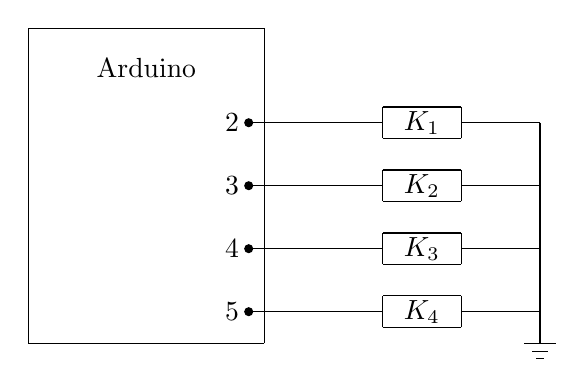
\begin{tikzpicture}
            % La carte arduino
            \draw (-1.5,2) -- (1.5,2);
            \draw (1.5,2) -- (1.5,-2);
            \draw (1.5,-2) -- (-1.5,-2);
            \draw (-1.5,-2) -- (-1.5,2);
            \draw (0,1.5) node {Arduino};

            % Pins
            \filldraw (1.3,.8) circle [radius=.05] node [left] {$2$};
            \filldraw (1.3,0) circle [radius=.05] node [left] {$3$};
            \filldraw (1.3,-.8) circle [radius=.05] node [left] {$4$};
            \filldraw (1.3,-1.6) circle [radius=.05] node [left] {$5$};

            % K1
            \draw (1.3,.8) -- (3,.8);
            \draw (3,.6) -- (3,1);
            \draw (3,1) -- (4,1);
            \draw (4,1) -- (4,.6);
            \draw (4,.6) -- (3,.6);
            \draw (3.5,.8) node {$K_1$};
            \draw (4,.8) -- (5,.8);

            % K2
            \draw (1.3,0) -- (3,0);
            \draw (3,-.2) -- (3,.2);
            \draw (3,.2) -- (4,.2);
            \draw (4,.2) -- (4,-.2);
            \draw (4,-.2) -- (3,-.2);
            \draw (3.5,0) node {$K_2$};
            \draw (4,0) -- (5,0);

            % K3
            \draw (1.3,-.8) -- (3,-.8);
            \draw (3,-.6) -- (3,-1);
            \draw (3,-1) -- (4,-1);
            \draw (4,-1) -- (4,-.6);
            \draw (4,-.6) -- (3,-.6);
            \draw (3.5,-.8) node {$K_3$};
            \draw (4,-.8) -- (5,-.8);

            % K4
            \draw (1.3,-1.6) -- (3,-1.6);
            \draw (3,-1.8) -- (3,-1.4);
            \draw (3,-1.8) -- (4,-1.8);
            \draw (4,-1.8) -- (4,-1.4);
            \draw (4,-1.4) -- (3,-1.4);
            \draw (3.5,-1.6) node {$K_4$};
            \draw (4,-1.6) -- (5,-1.6);

            % Ground
            \draw (5,.8) -- (5,-2);
            \draw (4.8,-2) -- (5.2,-2);
            \draw (4.9,-2.1) -- (5.1,-2.1);
            \draw (4.95,-2.2) -- (5.05,-2.2);
        \end{tikzpicture}
    \end{center}
\end{frame}

\begin{frame}
    \frametitle{Circuit de contrôle.}
    \framesubtitle{Partie puissance.}
    \begin{center}
        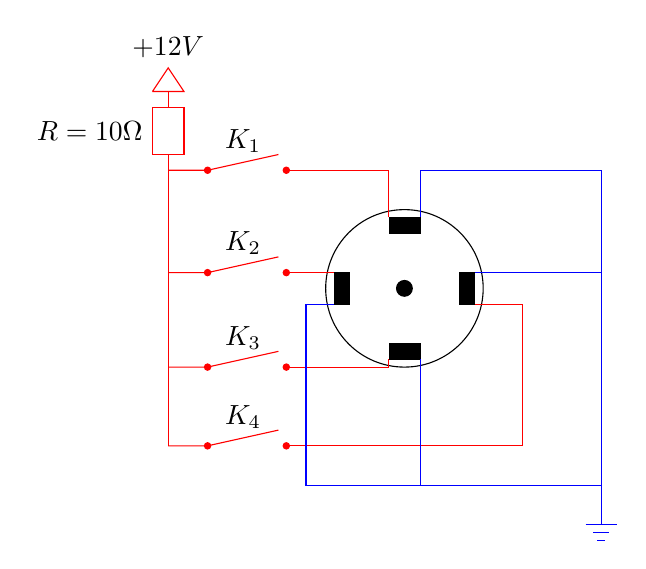
\begin{tikzpicture}
            % Le motor
            \draw (0,0) circle [radius=1];
            \filldraw (0,0) circle [radius=.1];
            \filldraw (-.2,.9) -- (.2,.9) -- (.2,.7) -- (-.2,.7);
            \filldraw (-.2,-.9) -- (.2,-.9) -- (.2,-.7) -- (-.2,-.7);
            \filldraw (-.9,.2) -- (-.7,.2) -- (-.7,-.2) -- (-.9,-.2);
            \filldraw (.9,.2) -- (.7,.2) -- (.7,-.2) -- (.9,-.2);

            % Command
            \draw[red] (-3.2,2.5) -- (-2.8,2.5) -- (-3,2.8) node [above,black] {$+12V$} -- (-3.2,2.5);
            \draw[red] (-3.2,1.7) -- (-2.8,1.7) -- (-2.8,2.3) -- (-3.2,2.3) -- node [left,black] {$R=10\Omega$} (-3.2,1.7);
            \draw[red] (-3,2.3) -- (-3,2.5);
            \draw[red] (-3,1.7) -- (-3,-2);
            % K1
            \draw[red] (-3,1.5) -- (-2.5,1.5) -- node [above,black] {$K_1$} (-1.6,1.7);
            \filldraw[red] (-2.5,1.5) circle [radius=.04];
            \filldraw[red] (-1.5,1.5) circle [radius=.04];
            \draw[red] (-1.5,1.5) -- (-.2,1.5) -- (-.2,.9);
            % K2
            \draw[red] (-3,.2) -- (-2.5,.2) -- node [above,black] {$K_2$} (-1.6,.4);
            \filldraw[red] (-2.5,.2) circle [radius=.04];
            \filldraw[red] (-1.5,.2) circle [radius=.04];
            \draw[red] (-1.5,.2) -- (-.9,.2);
            % K3
            \draw[red] (-3,-1) -- (-2.5,-1) -- node [above,black] {$K_3$} (-1.6,-.8);
            \filldraw[red] (-2.5,-1) circle [radius=.04];
            \filldraw[red] (-1.5,-1) circle [radius=.04];
            \draw[red] (-1.5,-1) -- (-.2,-1) -- (-.2,-.9);
            % K4
            \draw[red] (-3,-2) -- (-2.5,-2) -- node [above,black] {$K_4$} (-1.6,-1.8);
            \filldraw[red] (-2.5,-2) circle [radius=.04];
            \filldraw[red] (-1.5,-2) circle [radius=.04];
            \draw[red] (-1.5,-2) -- (1.5,-2) -- (1.5,-.2) -- (.9,-.2);

            % Ground
            \draw[blue] (.2,.9) -- (.2,1.5) -- (2.5,1.5);
            \draw[blue] (.9,.2) -- (2.5,.2);
            \draw[blue] (.2,-.9) -- (.2,-2.5);
            \draw[blue] (-.9,-.2) -- (-1.25,-.2) -- (-1.25,-2.5) -- (2.5,-2.5);
            \draw[blue] (2.5,1.5) -- (2.5,-3);
            \draw[blue] (2.3,-3) -- (2.7,-3);
            \draw[blue] (2.4,-3.1) -- (2.6,-3.1);
            \draw[blue] (2.45,-3.2) -- (2.55,-3.2);
        \end{tikzpicture}
    \end{center}
\end{frame}

\subsection{Propulsion.}
\begin{frame}
    \frametitle{Choix du moteur.}
    \begin{exampleblock}{Performance voulues.}
        \[ P = 80W \]
        \[ \omega = 870rad.s^{-1} \]
    \end{exampleblock}
    \only<2-> {
        \begin{block}{Caractéristiques du moteur choisit.}
            \begin{itemize} % TODO
                \item $U = 12V$
                \item $I = 0.6A$
                \item $P = 7.2W$.
                \item $\omega = xxrad.s^{-1}$.
            \end{itemize}
        \end{block}
    }
\end{frame}

